% Single editable source: main.tex. Compile with XeLaTeX. Keep figures/ beside this file.
% Chapters, table data and bibliography are inlined below; no BibTeX step is needed.
\documentclass[11pt,a4paper,oneside]{report}
\usepackage[top=25.4mm,bottom=25.4mm,left=25.4mm,right=24.9767mm,footskip=12.49mm]{geometry}
\usepackage{fontspec}
\IfFontExistsTF{Calibri}{\setmainfont{Calibri}}{\IfFontExistsTF{Carlito}{\setmainfont{Carlito}}{\setmainfont{TeX Gyre Heros}}}
\IfFontExistsTF{Times New Roman}{\newfontfamily\coverfont{Times New Roman}}{\newfontfamily\coverfont{TeX Gyre Termes}}
\IfFontExistsTF{Consolas}{\setmonofont{Consolas}[Scale=MatchLowercase]}{\setmonofont{lmmono10-regular.otf}[Scale=MatchLowercase]}
\usepackage[english]{babel}
\usepackage{amsmath,amssymb,booktabs,tabularx,longtable,array,multirow}
\usepackage[table]{xcolor}
\usepackage{graphicx}
\usepackage{titlesec,setspace,enumitem,caption,float,placeins,fvextra}
\usepackage[round,authoryear]{natbib}
\usepackage{xurl}
\usepackage[unicode,colorlinks=true,linkcolor=black,citecolor=black,urlcolor=navy,bookmarksnumbered=true]{hyperref}
\definecolor{chapterred}{HTML}{C00000}
\definecolor{navy}{HTML}{254B70}
\definecolor{teal}{HTML}{187E83}
\definecolor{orange}{HTML}{C96F21}
\definecolor{purple}{HTML}{79559A}
\definecolor{pale}{HTML}{F2F5F7}
\definecolor{peach}{HTML}{FCE8E0}
\renewcommand{\thechapter}{\Roman{chapter}}
\renewcommand{\thesection}{\arabic{section}}
\renewcommand{\thesubsection}{\arabic{section}.\arabic{subsection}}
\renewcommand{\thefigure}{\arabic{figure}}
\renewcommand{\thetable}{\arabic{table}}
\usepackage{chngcntr}
\counterwithout{figure}{chapter}\counterwithout{table}{chapter}
\titleformat{\chapter}[hang]{\color{chapterred}\bfseries\fontsize{16}{19}\selectfont}{\thechapter.}{.5em}{}
\titleformat{\section}{\bfseries\fontsize{13}{16}\selectfont}{\thesection.}{.5em}{}
\titleformat{\subsection}{\bfseries\fontsize{12}{15}\selectfont}{\thesubsection}{.5em}{}
\titlespacing*{\chapter}{0pt}{0pt}{12pt}
\titlespacing*{\section}{0pt}{12pt}{5pt}
\titlespacing*{\subsection}{0pt}{10pt}{4pt}
\setstretch{1.15}
\setlength{\parindent}{0pt}\setlength{\parskip}{4pt}
\raggedbottom
\renewcommand{\contentsname}{Table of Contents}
\setlength{\emergencystretch}{2em}
\setlength{\tabcolsep}{5pt}
\renewcommand{\arraystretch}{1.22}
\setlist{nosep,leftmargin=1.5em,topsep=4pt}
\captionsetup{font=small,labelfont=bf,skip=7pt}
\hypersetup{pdftitle={Retrieval-Augmented Question Answering for Vietnamese Legal Documents},pdfauthor={Group 4, FPT University},pdfsubject={Data Science Project: implementation and development benchmark}}
\newcolumntype{Y}{>{\raggedright\arraybackslash}X}
\newcolumntype{P}[1]{>{\raggedright\arraybackslash}p{#1}}
\newcommand{\code}[1]{\texttt{\detokenize{#1}}}
\newcommand{\note}[1]{\par\smallskip{\small\textit{#1}}\par}
\newcommand{\frontchapter}[1]{\chapter*{#1}\addcontentsline{toc}{chapter}{#1}}
\newenvironment{reporttable}{\begin{center}\small}{\end{center}}
\DefineVerbatimEnvironment{commands}{Verbatim}{fontsize=\footnotesize,breaklines=true,breakanywhere=true,frame=single,rulecolor=\color{gray!40},framesep=5pt}
\begin{document}
% BEGIN chapters/front
\hypersetup{pageanchor=false}
\begin{titlepage}
\thispagestyle{empty}
\begin{minipage}[c]{.33\textwidth}
\includegraphics[width=4cm]{figures/fpt-logo.png}\end{minipage}\hfill
\begin{minipage}[c]{.64\textwidth}\centering\bfseries\fontsize{14}{17}\selectfont MINISTRY OF EDUCATION AND TRAINING\end{minipage}
\vspace{1.8cm}
\begin{center}
{\fontsize{30}{36}\selectfont\bfseries FPT UNIVERSITY}\par
\vspace{2.0cm}
{\coverfont\fontsize{25}{30}\selectfont Data Science Project Document}\par
\vspace{.35cm}
{\color{navy}\rule{\textwidth}{.4pt}}\par
{\coverfont\fontsize{20}{24}\selectfont Retrieval-Augmented Question Answering for Vietnamese Legal Documents}\par
\vspace{1.1cm}
\renewcommand{\arraystretch}{1.45}
\begin{tabularx}{.98\textwidth}{|>{\raggedleft\arraybackslash\bfseries}p{4.4cm}|Y|}
\hline
\multicolumn{2}{|c|}{\large\bfseries Group 4}\\\hline
\multirow{4}{4.4cm}{\raggedleft\bfseries Group Members} & Vo Tran Ngoc Trung\hfill SE192927\\
& Nguyen Tri Anh\hfill SE192569\\
& Nguyen Thanh Luan\hfill SE193674\\
& Nguyen Duc Anh\hfill SE196482\\\hline
Supervisor & Nguyen Trong Tai\\\hline
Project Code & N/A\\\hline
\end{tabularx}
\vfill
Ho Chi Minh City, November 2026
\end{center}
\end{titlepage}
\pagenumbering{roman}
\hypersetup{pageanchor=true}
\setcounter{tocdepth}{1}
\renewcommand{\contentsname}{Table of Contents}
\tableofcontents
\frontchapter{Acknowledgement}
We thank our supervisor, Nguyen Trong Tai, and FPT University for the academic setting in which this Data Science Project was developed. We also acknowledge the researchers and maintainers who made the retrieval methods, pretrained models, open-source infrastructure, and public legal-text collection used in this project available. Responsibility for the implementation, interpretation of the experiments, and remaining limitations rests with the project team.

\par\bigskip\phantomsection{\color{chapterred}\bfseries\fontsize{16}{19}\selectfont Definition and Acronyms}\par
\addcontentsline{toc}{chapter}{Definition and Acronyms}
\begin{reporttable}
\begin{tabularx}{\textwidth}{lY}
\toprule\textbf{Term} & \textbf{Meaning in this report}\\\midrule
AI / NLP & Artificial Intelligence / Natural Language Processing.\\
RAG & Retrieval-Augmented Generation: generation conditioned on retrieved external evidence.\\
Graph-assisted RAG & Source-backed document-reference traversal added to retrieval in this implementation.\\
LLM & Large Language Model.\\
BM25 & A lexical ranking function from probabilistic information retrieval.\\
RRF & Reciprocal Rank Fusion, combining rankings using reciprocal ranks.\\
HNSW & Hierarchical Navigable Small World approximate nearest-neighbour index.\\
IR / qrels & Information Retrieval / question-to-relevant-chunk judgments.\\
MRR / MAP & Mean Reciprocal Rank / Mean Average Precision.\\
nDCG & Normalized Discounted Cumulative Gain.\\
Faithfulness & Proportion of extracted answer claims judged supported by supplied context.\\
Factual F1 & Per-question harmonic mean of reference-based claim precision and recall.\\
CI / WBS & Confidence Interval / Work Breakdown Structure.\\
Development set & Questions used during pipeline improvement; not a held-out final test.\\
\bottomrule
\end{tabularx}
\end{reporttable}
\clearpage
\listoftables\addcontentsline{toc}{chapter}{List of Tables}
\clearpage
\listoffigures\addcontentsline{toc}{chapter}{List of Figures}
\clearpage
\pagenumbering{arabic}
% END chapters/front

% BEGIN chapters/introduction
\chapter{Project Introduction}\label{ch:introduction}
\section{Overview}
\subsection{Project Information}
\begin{table}[H]\centering\small
\caption{Project identity and documented team membership.}\label{tab:team}
\begin{tabularx}{\textwidth}{lYl}\toprule
\textbf{No.} & \textbf{Full name} & \textbf{Student code}\\\midrule
1 & Vo Tran Ngoc Trung & SE192927\\
2 & Nguyen Tri Anh & SE192569\\
3 & Nguyen Thanh Luan & SE193674\\
4 & Nguyen Duc Anh & SE196482\\\bottomrule
\end{tabularx}
\end{table}
The project, \textit{Retrieval-Augmented Question Answering for Vietnamese Legal Documents}, is undertaken by Group 4 under the supervision of Nguyen Trong Tai at FPT University. No separate project code is recorded. Its domain combines natural language processing, legal information retrieval, and evaluation of generative systems. Intended users include students, researchers, and readers seeking to locate provisions and understand the content of supplied legal documents.

\subsection{Project Overview}
The project implements a Vietnamese legal question-answering pipeline that connects a natural-language question to traceable source passages. It combines lexical and dense retrieval, optionally expands candidates through a document-reference graph, and optionally reranks the results. A context builder retains complete legal evidence within a token budget. An online evaluator checks whether that evidence is sufficient before the answer generator is called. A separate verifier then checks the generated citations and their support. If these checks do not pass, the system can return an explicit fallback rather than a completed answer.

The research contribution is an inspectable implementation and a controlled benchmark across five retrieval configurations. The evidence reported here consists of a frozen development run of 45 questions and 225 pipeline executions. It supports analysis of operational behaviour, retrieval, context quality, answer quality, and inference latency. It does not establish legal correctness for unseen cases or superiority over commercial legal assistants.

\begin{figure}[H]\centering
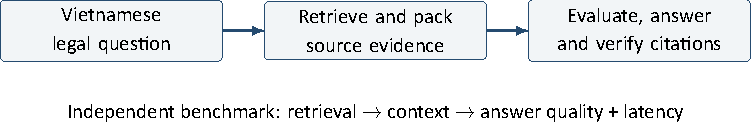
\includegraphics{figures/rendered/figure-01.pdf}
\caption{Project objective: evidence-linked answering with a separate evaluation workflow.}\label{fig:objective}
\end{figure}

\section{Project Background}
Legal retrieval requires attention to document identity and to the relationship between an article, its clauses, and their conditions. A passage containing the right subject words may describe a narrower scope than the question asks for. Conversely, an answer can be incomplete when retrieval finds the correct article but omits an exception or a second required document. These are distinct problems of ranking, evidence coverage, and reasoning over retained text.

RAG conditions generation on retrieved material rather than relying exclusively on model parameters \citep{lewis2020rag}. That design provides an evidence channel, but does not by itself guarantee that the right material is retrieved or that every generated statement follows from it. The present implementation therefore treats retrieval, context sufficiency, and answer verification as separate responsibilities. This separation also makes failures easier to diagnose: a ranking miss should not be conflated with a citation mismatch or an unreliable offline judge.

The data source is a pinned snapshot of a community-hosted mirror of Vietnamese codified legal texts \citep{phapdien}. Source URLs and revision identifiers are preserved for traceability. A source-backed amendment or replacement link can help discover a related document, but its presence alone does not prove the law applicable to a particular date or dispute. Temporal legal interpretation remains outside the guarantees of this prototype.

\section{Project Objective}
The first objective is to implement an end-to-end, modular pipeline that produces an answer supported by retained passages, or a clear insufficient-evidence outcome. The second is to compare a hybrid baseline with reranking, graph assistance, and bounded retrieval feedback under shared data, models, and budgets. The third is to report inference cost alongside quality so that a small numerical improvement is considered together with its latency and uncertainty.

These objectives are operationalized through the research questions in Chapter~\ref{ch:methodology}. Success means that the workflow can be reproduced, its evidence and failures can be inspected, and conclusions respect the limitations of the experiment. It does not mean that every completed response is legally correct or that adding more components must improve performance.

\section{Problem Statement}
Given a question $q$ and a fixed legal corpus $D$, the system must select evidence $C\subset D$ under a context budget and return an answer $a$ with source-linked citations. The challenge is to preserve the question's scope while balancing exact legal identifiers, semantic similarity, graph neighbours, and limited generation context. The benchmark asks whether each optional component improves retrieval or downstream quality relative to the same hybrid baseline, and what additional latency is observed.

Three sources of uncertainty must remain visible. First, the relevance labels cover identified evidence rather than all potentially useful passages. Second, development questions have informed pipeline changes. Third, several quality measures rely on model judgments that can themselves be inconsistent. A defensible report must describe these limitations instead of treating a single aggregate score as the system's accuracy.

\section{Significance of the Project}
The project connects source provenance with experimental observability. Hierarchical chunks retain legal locations, the generator selects from numbered retained sources, and citation identities and quotations are constructed from those sources. The benchmark stores the resulting ranks, packed context, decisions, answers, timings, and judgment details. This makes it possible to investigate why a result occurred and to separate engineering reliability from evidence of retrieval effectiveness.

For the course, the work illustrates a complete data science process: data selection and preparation, representation design, controlled ablation, quantitative analysis, and critical interpretation. The practical output is a reproducible research prototype and benchmark tooling. Independent legal review and broader evaluation would be required before making stronger claims about deployment readiness.

\section{Project Scope \& Limitations}
\subsection{Project Scope}
\textbf{A. Data and domain.} The evaluated corpus covers three selected topics: transportation and traffic, science and technology, and education and training. It contains 7,425 source article records originating from 647 documents. These are transformed into 14,708 embedded leaf chunks and 14,333 unembedded parent chunks. The report does not describe an experiment over the entire national legal corpus.

\textbf{B. Architecture and methods.} The implementation includes query analysis, deterministic metadata filtering, BM25 and dense retrieval, RRF, optional Neo4j graph retrieval, an optional cross-encoder reranker, hierarchical context packing, an online sufficiency gate, generation, and citation verification. Feedback is bounded to three retrieval rounds in B4. Graph traversal is independently bounded to depth two.

\textbf{C. Functionality.} The delivered interfaces are command-line preparation, question answering, interactive chat, diagnostics, and benchmark validation/run/score/report commands. A user-facing web application and live legal-update service are future extensions. The pipeline uses pretrained models through Ollama and an ONNX reranker; it does not fine-tune an LLM or train a reinforcement-learning policy.

\textbf{D. Evaluation.} The development pilot contains 45 answerable questions, evenly divided across three topics. It evaluates five configurations once each, with question-level pairing. Retrieval metrics use chunk relevance labels; context and answer metrics use a separate offline judge. Timings measure full pipeline inference under the recorded protocol, not corpus preparation or offline scoring.

\subsection{Limitations and Out-of-Scope}
The pilot is small and contains many explicit document or provision cues. Its labels have not been independently reviewed by legal experts, and the same questions have supported development. There are no held-out final-test or unanswerable questions in this run. Dense retrieval quality is not isolated from the other shared pipeline components, and no chunking or model-family ablation is included.

The snapshot does not establish current legal validity. Citation verification constrains the evidence channel but is not a formal proof that every sentence is entailed. The offline judge has truncation errors and demonstrable semantic inconsistencies. Incomplete hardware and LLM quantization records limit the portability of latency results.
% END chapters/introduction

% BEGIN chapters/management
\chapter{Project Management Plan}
\section{Team Work}
\subsection{Team Structure and Roles}
Table~\ref{tab:team} records the four members supplied in the course document. Individual role assignments, time sheets, and a signed responsibility allocation are not present in the inspected project artifacts. The report therefore describes responsibilities by work package rather than attributing undocumented work to particular students.

\begin{table}[H]\centering\small
\caption{Functional responsibilities and reviewable outputs.}\label{tab:responsibilities}
\begin{tabularx}{\textwidth}{P{3cm}YY}\toprule
\textbf{Responsibility} & \textbf{Engineering output} & \textbf{Review evidence}\\\midrule
Data preparation & Pinned source selection, normalized metadata, hierarchical chunks & Corpus manifest, source revision, chunk identities\\
Retrieval and context & Lexical/dense/graph candidates, fusion, reranking, packing & Ranking traces, retained source text, token budgets\\
Orchestration and reliability & Sufficiency decisions, bounded feedback, generation, verification & Status, round history, structured failures, regression tests\\
Evaluation and reporting & Question validation, scoring, statistics and visual analysis & Frozen run manifest, score artifacts, CSV/JSON exports\\\bottomrule
\end{tabularx}
\end{table}
These responsibilities provide a practical basis for peer review. Changes that cross boundaries should be reviewed against the relevant contracts: for example, a new chunk representation must remain compatible with evidence resolution, citation identity, and retrieval labels. Naming a module owner is useful for future coordination, but should be agreed by the team rather than inferred from this report.

\subsection{Communication Plan}
The recommended communication process is to maintain implementation issues and benchmark findings with the code repository. Each issue should identify a concrete input, the observed behaviour, the expected contract, and the artifact needed to reproduce it. A short integration review at each work-package boundary should resolve configuration or schema changes before the next complete benchmark.

This is a proposed working process; the repository does not supply meeting minutes or evidence of a fixed weekly meeting schedule. For academic review, the supervisor can assess the documented architecture, experiment matrix, and result interpretation. Decisions affecting labels or legal scope should be recorded separately from implementation fixes so that later runs can distinguish data changes from system changes.

\section{Project Management Approach}
\subsection{Work Breakdown Structure}
The work is organized by dependency rather than by an invented calendar. Figure~\ref{fig:wbs} shows the sequence of deliverable gates. A corpus snapshot must be identifiable before evidence labels can be checked; inference artifacts must be frozen before offline judgments and statistical summaries can be audited.

\begin{figure}[H]\centering
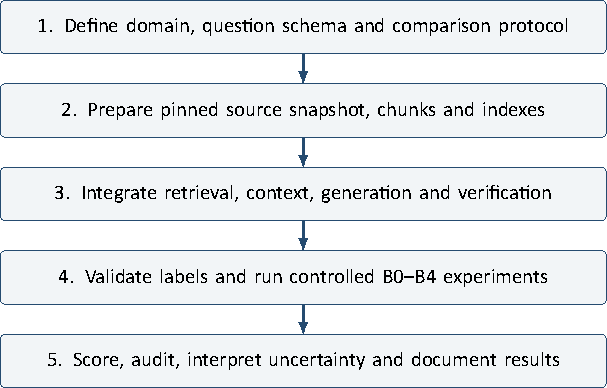
\includegraphics{figures/rendered/figure-02.pdf}
\caption{Work-package dependencies and review gates. This is a delivery structure, not a record of dates.}\label{fig:wbs}
\end{figure}

\subsection{Risk Management}
\begin{table}[H]\centering\small
\caption{Material risks and controls supported by the project design.}\label{tab:risks}
\begin{tabularx}{\textwidth}{P{3.1cm}YY}\toprule
\textbf{Risk} & \textbf{Control} & \textbf{Residual limitation}\\\midrule
Missing scope or conditions & Preserve original-question filters; retain complete parent evidence where budget allows & Correct ranking may still omit required provisions\\
Fabricated citations & Source-number selection and deterministic citation construction; support verifier & Model-based verification can misjudge entailment\\
Source/version drift & Pin dataset revision and corpus identity; preserve source URLs & Snapshot does not certify current legal effect\\
Benchmark leakage & Declare development use; separate future held-out test & Existing pilot cannot be treated as unseen evaluation\\
Judge bias and truncation & Store claim judgments and errors; report valid denominators & Current quality means remain provisional\\
Slow or interrupted runs & Cache prepared corpus; atomic sample artifacts and resume checks & Model loading and local contention affect timings\\\bottomrule
\end{tabularx}
\end{table}
Risk management should prioritize observed failure modes. In this pilot, context-sufficiency false negatives and offline judge instability are more actionable than hypothetical increases in graph complexity. Their fixes require separate controls so that improving the evaluator does not silently change the underlying relevance labels.

\subsection{Quality Management}
Quality is checked at three levels. Deterministic tests enforce schemas, metadata matching, token budgets, source integrity, and failure handling. Focused regression cases exercise the interaction between retrieval scope, context packing, and citation verification. The benchmark then compares end-to-end behaviour under a shared protocol. Passing one level does not establish the next: a valid JSON response may still be unsupported, and a successful regression case is not a held-out accuracy estimate.

The latest recorded project-wide regression run contains 366 passed tests, 10 skipped tests, and 246 subtests. Two focused post-fix inference batches contain 11 B3 cases and four B0 cases, all completed, while two missing-evidence controls were rejected. These checks support the stability of the revised contracts. They are development checks, not independent experimental evidence of general legal-answering accuracy.

\subsection{Budget and Funding}
No expenditure ledger, paid-service budget, or measured energy cost is included in the project evidence. The prototype uses open-source software and locally served pretrained models. This removes the need to report an assumed commercial API bill, but does not make computation cost-free. Hardware ownership, electricity, model storage, and researcher time remain unmeasured. Future cost reporting should record these quantities together with the number of completed and judged questions.

\subsection{Change Management Process}
A meaningful change should include an explicit reason and a narrow verification case. Retrieval or orchestration changes should be checked against the original question, retained evidence, and final citation behaviour. Dataset edits require a new version and a documented explanation. A complete comparison should use a new output directory so that artifacts from different code or label versions are not mixed.

The run manifest stores configuration, code identity, model identities, question contents, and the latency protocol. The scorer stores its own identity and fingerprints. These records support an auditable chain from the selected source snapshot to a reported number. They do not replace a clean code snapshot: the report is based on the current working project and frozen artifacts, and its regeneration instructions preserve the distinction between rebuilding a document and rerunning inference.

\subsection{Closure and Evaluation}
The present milestone closes with a working benchmark cycle and a documented development result. Closure requires that all 225 expected sample and score artifacts are accounted for, report tables agree with those artifacts, and unresolved issues are stated. The next research milestone should require an independently reviewed held-out set, more complete hardware records, and calibration of the offline judge. A statistically significant advantage is not a prerequisite for an academically useful result; transparent evidence that a proposed addition did not demonstrate a benefit is itself informative.
% END chapters/management

% BEGIN chapters/related
\chapter{Existing Systems/State of the Art}
\section{Overview of the Field}
Question answering over a specialist corpus involves two related but separate tasks: locating relevant information and producing an explanation that follows from it. Traditional retrieval exposes ranked documents or passages directly. Generative systems add a natural-language synthesis step, which can help users read the evidence but also introduces statements that require verification. For legal material, document numbers, provision boundaries, and qualification clauses make this distinction particularly consequential.

The present project belongs to retrieval-augmented question answering. Its comparison is internal: the same hybrid retrieval baseline is augmented with optional reranking, graph traversal, and feedback. This report reviews the methods that motivate those additions without transferring published performance claims to the Vietnamese development corpus.

\section{Historical Context}
Lexical retrieval, represented here by BM25, ranks documents using term evidence and length normalization \citep{robertson2009bm25}. It is useful when a query contains exact legal names or identifiers. Dense retrieval represents text in a learned vector space and can match related wording even when terms differ. Combining the two is a reasonable design hypothesis because exact and semantic matching can fail in different ways.

RAG introduced a prominent framework for conditioning language generation on retrieved non-parametric information \citep{lewis2020rag}. The original research includes model training and experiments on knowledge-intensive NLP tasks. This project borrows the retrieval-conditioned design principle while using frozen pretrained inference models; it does not reproduce the original training procedure or evaluation datasets.

\section{Key Studies and Theories}
\subsection{Retrieval Fusion and Ranking}
RRF combines ranked lists by summing reciprocal rank contributions \citep{cormack2009rrf}. Its appeal here is that BM25 scores, cosine similarities, and graph-derived ranks need not be placed on a common numerical scale. The method rewards candidates supported by several lists, while retaining contributions from a single retriever. This is a motivation for its use, not a guarantee of a gain for every corpus.

Ranking should also be evaluated in more than one way. Recall measures whether labeled evidence is found, reciprocal rank emphasizes the first relevant hit, and average precision accounts for all labeled hits. nDCG discounts relevance lower in the list and normalizes against an ideal ranking \citep{jarvelin2002gain}. The project uses binary chunk relevance, so it does not evaluate graded legal authority or graded degrees of usefulness.

\subsection{Multilingual Representations and Legal Structure}
M3-Embedding supports multilingual text representations and several retrieval modes \citep{chen2024m3}. The project uses only the dense representation of BGE-M3. Its separate BM25 component is not the learned sparse mode of that model. Therefore, calling the implementation ``BGE-M3 hybrid retrieval'' would obscure the actual combination being tested.

The cross-encoder model card describes a multilingual mMARCO-trained query--passage ranker \citep{mmarco}. A cross-encoder evaluates a question and candidate jointly rather than relying only on independently stored vectors. The implementation runs a pinned ONNX int8 export. Published multilingual capabilities do not establish Vietnamese legal-domain calibration, especially for long provisions truncated to the configured 512-token reranker input.

Legal hierarchy motivates a complementary representation choice. A leaf may be appropriate for retrieval, while a complete clause or article is needed for answering. This project explicitly separates embedded leaves from unembedded parents. The current experiment fixes that representation for every method; it provides no causal estimate that hierarchical chunking is superior to fixed windows.

\subsection{Corpus Provenance}
The collection is obtained from the \code{tmquan/phapdien-moj-gov-vn} dataset mirror \citep{phapdien}. Ingestion records the resolved source commit and preserves document and provision metadata. The benchmark uses a selected three-topic corpus, not the entire dataset. A provenance record makes the experiment repeatable at a given snapshot, but does not certify that the mirror is complete, legally reviewed, or up to date.

\section{Technological Advancements}
\subsection{Graph-Based Retrieval}
Graph approaches can expose relationships that a passage-only ranking may not directly surface. However, ``Graph RAG'' covers different architectures. \citet{edge2024graph} describe an LLM-built entity graph with community summaries for global, query-focused summarization. The implementation in this project instead uses explicit document references and source-backed typed links, plus a hierarchy of legal chunks. It has no community detection, community summaries, or global map--reduce synthesis.

This distinction determines the experiment's interpretation. Enabling the graph branch tests whether bounded document-neighbour expansion adds useful candidates. It does not reproduce Microsoft GraphRAG or test its published global sensemaking setting. The pilot also needs questions that actually depend on available graph links before it can substantiate a graph-specific benefit.

\subsection{Context and Answer Evaluation}
RAGAs motivates evaluating different stages of a RAG pipeline rather than relying on a single answer score \citep{es2024ragas}. This project implements its own Ragas-style context and answer measures with stored judgment details. It does not call the RAGAs package, and numerical values should not be assumed interchangeable with a particular library version or prompt set.

ARES similarly treats evaluation as a measurement problem, using learned judges and human annotation to improve estimation \citep{saadfalcon2024ares}. Its relevance here is methodological: a model judge needs calibration and validation. The project does not implement ARES or its training procedure. Its own recorded judge disagreements make independent human review a necessary next step.

\section{Comparison of Existing Systems}
Table~\ref{tab:related} compares architectural capabilities. It is not an empirical leaderboard, and does not assign scores to untested public or commercial systems.

\begin{table}[H]\centering\small
\caption{Conceptual comparison of retrieval and answering approaches.}\label{tab:related}
\begin{tabularx}{\textwidth}{P{2.5cm}YYY}\toprule
\textbf{Approach} & \textbf{Evidence access} & \textbf{Typical strength} & \textbf{Limitation relevant here}\\\midrule
Lexical retrieval & Term-matched documents/passages & Exact identifiers and terminology & Wording mismatch; no answer synthesis\\
Dense retrieval & Nearest vector representations & Semantic matching & Can blur exact scope and identifiers\\
Hybrid RAG & Fused candidates and generated answer & Combines lexical and semantic evidence & Generation may exceed evidence\\
Community GraphRAG & Entity graph and community summaries & Corpus-level thematic synthesis & Different task and graph construction\\
This prototype & Hybrid ranks; optional document graph; packed provisions & Traceable local evidence and observable gates & Pilot-limited coverage and uncalibrated judge\\\bottomrule
\end{tabularx}
\end{table}

\section{Gaps in Literature/Technology}
General retrieval and RAG research does not determine how well a particular legal snapshot, tokenizer, model, and prompt combination will work. The project therefore addresses an applied evidence gap: a reproducible comparison of these components on a Vietnamese legal pilot with explicit source labels. A second gap is operational observability. Ranking improvements can disappear when context packing drops a required condition or when a sufficiency gate rejects an otherwise answerable question.

The current evidence exposes a further measurement gap. A semantic judge can penalize a faithful scope statement because it expects details absent from the question. Such errors are not resolved by collecting more model-generated scores alone. The benchmark must retain inspectable judgments and eventually compare them with independently adjudicated legal evidence.

\section{Justification for the Project}
The chosen architecture makes these questions testable within a course project. Lexical and vector retrieval provide a shared baseline. Graph retrieval and reranking can be switched independently. Context packing and online evaluation remain common, and all outputs are captured before offline scoring. This design supports incremental engineering and controlled ablation without claiming a new foundation model or a complete legal reasoning system.
% END chapters/related

% BEGIN chapters/methodology
\chapter{Methodology}\label{ch:methodology}
\section{Research Questions and Objectives}
The experiment is a controlled development-set ablation. It asks:
\begin{enumerate}
\item Does a cross-encoder improve the ranked evidence and downstream context relative to hybrid BM25 plus dense retrieval?
\item Does bounded traversal of source-backed document links add useful evidence beyond the same hybrid baseline?
\item Does combining graph retrieval and reranking improve quality enough to justify its observed inference latency?
\item When the context gate rejects evidence, does bounded retrieval feedback recover additional completed answers?
\end{enumerate}
These questions concern the implemented system and selected corpus. They are not hypotheses about all Vietnamese legal tasks. The study records quality at three stages and timing separately, rather than choosing a winner from one unqualified composite score.

\section{Data Collection and Preprocessing}
\subsection{Source Selection and Representation}
The prepared corpus resolves the source dataset to commit
\begin{quote}\small\path{a1b6860c821b7142ffe2385178af4e4bb6f86aff}.\end{quote}
Its local corpus identity is \code{4d70694000eb63e3}. Selection retains 7,425 article records from 647 originating documents in three topics. Metadata includes source dataset and revision, document identifiers and numbers, source URLs, and available article/clause/point locations. Unknown legal status is retained as unknown rather than interpreted as currently effective.

The hierarchical chunker uses a 512-token target and 64-token overlap for fallback token windows. It preserves article roots, recognizes numbered clauses, and splits long clauses into points when numbering is unambiguous. Ambiguous or oversized segments fall back to token windows. Heading context accompanies leaves. Parents are stored for later context expansion but are not embedded. This produces 14,708 embedded leaves and 14,333 parent chunks.

\begin{figure}[H]\centering
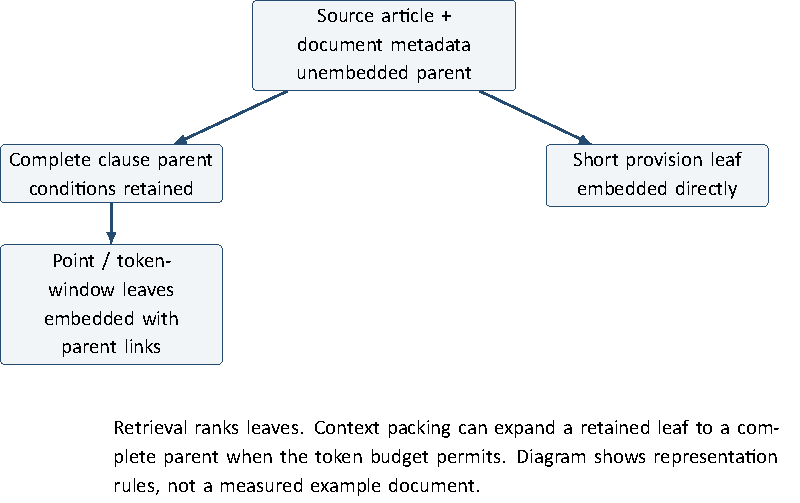
\includegraphics{figures/rendered/figure-03.pdf}\vspace{10mm}
\caption{Hierarchical representation separates retrieval granularity from answering context.}\label{fig:hierarchy}
\end{figure}

\subsection{Question Set and Evidence Labels}
The normalized file \code{three_topics_pilot.development.v1.jsonl} contains 45 questions: 15 per topic. Question types are shown in Figure~\ref{fig:types}. Each record contains a stable identifier, Vietnamese question, reference answer, atomic reference claims, and source evidence with document identity, legal location, and an exact quotation. There are 233 reference claims and 115 evidence spans. All labeled spans resolve against the prepared corpus.

\begin{figure}[H]\centering
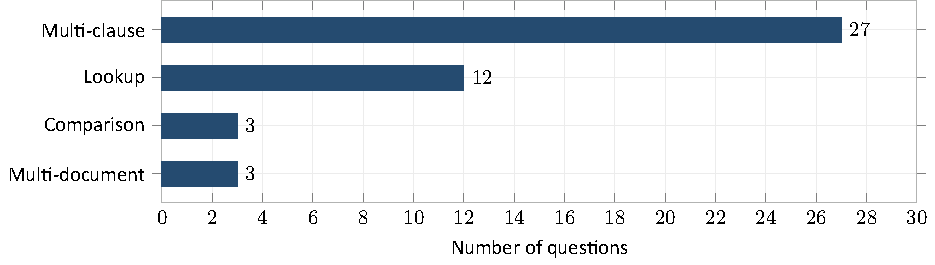
\includegraphics{figures/rendered/figure-04.pdf}
\caption{Development-set composition: 45 questions, all labeled answerable; three topics contribute 15 questions each.}\label{fig:types}
\end{figure}

Twelve question wordings were clarified during development to align the requested scope with the recorded evidence. The original draft is preserved separately. The normalized file is therefore a development artifact, and the report does not treat the questions as a held-out test. The labels remain pending independent legal review.

The evidence resolver normalizes Unicode NFC and whitespace and matches quotations within the labeled document and provision location. It produces binary relevant leaf IDs. A leaf overlapping the exact labeled quote can be relevant, but alternative useful provisions are not exhaustively labeled. In this run, 39 questions have one relevant leaf and six have two. This narrow labeling scheme is essential to interpreting precision.

\section{Feature Selection and Engineering}
The project uses engineered representations and metadata rather than training tabular features. Lexical retrieval applies Unicode-aware, lowercase word tokenization and BM25Okapi with $k_1=1.2$ and $b=0.75$. Dense retrieval embeds question and leaf text into normalized 1,024-dimensional BGE-M3 vectors. Cosine search is served by pgvector HNSW. Exact document numbers and recognized legal locations are additional constraints, not embedding dimensions.

The original user question controls hard filters. LLM rewriting can improve retrieval wording, but cannot legitimately remove a document or condition from the request. Explicit document numbers are mapped to corpus vocabulary using deterministic normalization. Named article titles are used as hard constraints only when they can be resolved consistently for all referenced documents. Context prioritization can perform softer title matching and distribute candidates across requested documents, while leaving the recorded raw ranking intact for IR scoring.

For ranked lists $L_1,\ldots,L_m$, fusion assigns a candidate $d$ the score
\begin{equation}
\operatorname{RRF}(d)=\sum_{j:d\in L_j}\frac{1}{60+\operatorname{rank}_{L_j}(d)}.
\end{equation}
The optional reranker then scores query--candidate pairs. Graph candidates use the same metadata filters and enter fusion as an additional ranked list. The experiment fixes these shared rules so that the optional components can be compared without changing the source corpus or answer model.

\section{Model Training and Validation}
\subsection{Frozen Pretrained Inference}
No model is trained or fine-tuned in this study. The heading is retained from the course outline, but the relevant methodological choices are pretrained model selection, prompt configuration, and development validation. Table~\ref{tab:models} gives the measured-run roles. The online sufficiency evaluator and the offline quality judge have different responsibilities and must not be conflated.

\begin{table}[H]\centering\small
\caption{Models and budgets in the recorded development run.}\label{tab:models}
\begin{tabularx}{\textwidth}{P{3.5cm}YP{3cm}}\toprule
\textbf{Role} & \textbf{Model / backend} & \textbf{Key budget}\\\midrule
Dense embedding & BGE-M3 via Ollama & 1,024 dimensions\\
Query analysis & \code{qwen3.5:2b}, Ollama & 512 output tokens\\
Online context sufficiency & \code{qwen3.5:4b}, Ollama & 768 output tokens\\
Answer generation & \code{qwen3.5:4b}, Ollama & 2,048 output tokens\\
Citation support verification & \code{qwen3.5:2b}, Ollama & 512 output tokens\\
Optional reranking & mMARCO mMiniLMv2 L12 H384, ONNX int8 & 512 input tokens\\
Offline quality judging & \code{qwen3.5:2b}, Ollama & 2,048 output tokens\\\bottomrule
\end{tabularx}
\note{LLM context windows are 8,192 tokens; temperature is 0 and thinking is disabled. The offline judge differs from the generator model size, but shares the model family and the online verifier model. This is not independent human assessment.}
\end{table}

The reranker uses revision \code{1427fd652930e4ba29e8149678df786c240d8825}. The BGE-M3 tokenizer is pinned to revision \code{5617a9f61b028005a4858fdac845db406aefb181}. Model identities are captured in the run manifest. The configured backends and recorded digest are more informative than assuming the same mutable model tag always resolves to identical weights.

\subsection{Experimental Control}
\begin{table}[H]\centering\small
\caption{Controlled ablation matrix; every method includes BM25, dense retrieval and RRF.}\label{tab:matrix}
\begin{tabularx}{\textwidth}{lYccc}\toprule
\textbf{ID} & \textbf{Configuration} & \textbf{Graph} & \textbf{Rerank} & \textbf{Max. rounds}\\\midrule
B0 & Hybrid baseline & No & No & 1\\
B1 & Hybrid + reranker & No & Yes & 1\\
B2 & Hybrid + graph & Yes & No & 1\\
B3 & Hybrid + graph + reranker & Yes & Yes & 1\\
B4 & B3 + bounded refinement & Yes & Yes & 3\\\bottomrule
\end{tabularx}
\end{table}
All methods use 20 candidates per lexical/vector branch, a final ranked list of up to 20, and up to five packed context chunks. The context budget is 4,096 tokens with a 1,024-token prompt reserve. B4 preserves the configured methods and cutoffs across rounds; feedback refines the retrieval query rather than changing the ablation.

The run uses one repeat, seed 42, one excluded warm-up query per configuration, shuffled configuration order, and full query analysis for each timed execution. There are $45\times5=225$ expected executions. Warm-up reduces some startup effects but cannot remove local model-loading or scheduling variation. Neither repeated-run stability nor an independent test split is estimated by this pilot.

\section{Evaluation Metrics}
\subsection{Stage 1: Retrieval}
For question $q$, let $R_q$ be the unique labeled relevant leaf IDs and $z_i$ indicate whether the unique hit at rank $i$ belongs to $R_q$. For a cutoff $k$,
\begin{align}
P_q@k&=\frac{\sum_{i=1}^{k}z_i}{k},\\
R_q@k&=\frac{\sum_{i=1}^{k}z_i}{|R_q|},\\
RR_q@k&=\begin{cases}1/\min\{i\leq k:z_i=1\},&\text{if a relevant hit exists},\\0,&\text{otherwise},\end{cases}\\
AP_q@k&=\frac{\sum_{i=1}^{k}(P_q@i)z_i}{|R_q|},\\
DCG_q@k&=\sum_{i=1}^{k}\frac{z_i}{\log_2(i+1)},\\
nDCG_q@k&=\frac{DCG_q@k}{\sum_{i=1}^{\min(k,|R_q|)}1/\log_2(i+1)}.
\end{align}
Missing ranks contribute zero. The implementation deduplicates IDs while preserving order. MRR and MAP are macro means of $RR_q$ and $AP_q$, respectively; AP uses the total number of relevant IDs as its denominator, so missed labels remain misses. The report emphasizes $k=5$ and also reports recall at 20. It evaluates the final retained retrieval ranking for each question, not the context builder's reordered or expanded passages.

There are only 51 relevant question--leaf assignments across 45 questions. Even a perfect top-five ranking can therefore achieve at most
\begin{equation}
\overline{P@5}_{\max}=\frac{39\times1+6\times2}{45\times5}=0.2267.
\end{equation}
A precision value near 0.21 should be read against this label ceiling. It is neither a 21\% question-answer accuracy nor proof that every unlabeled retrieved passage is useless.

\subsection{Stage 2: Packed Context}
Let $v_i$ denote the offline judge's binary usefulness judgment for packed context chunk $i$, relative to the question and reference answer. Context Precision is rank-aware:
\begin{equation}
CP_q=\frac{\sum_{i=1}^{m}v_i\left(\sum_{j=1}^{i}v_j/i\right)}{\sum_{i=1}^{m}v_i},
\end{equation}
with zero when no context is judged useful. Its denominator counts useful \emph{retrieved} contexts. Consequently, a high score does not imply that all reference information was retrieved. It also differs from raw chunk-label $P@k$.

If the reference contains $s$ atomic claims and $u_j$ indicates whether claim $j$ is supported by the packed context, then Context Recall is $CR_q=\sum_j u_j/s$. These judgments operate on the actual packed text, including complete parent expansion when used. A correct leaf ID can be found while the semantic judge still considers the overall context incomplete.

\subsection{Stage 3: Answer Quality}
Faithfulness is the proportion of extracted answer claims judged supported by the supplied context. Factual precision is the fraction of response claims supported by the reference answer; factual recall is the fraction of reference claims covered by the response. Factual F1 is their harmonic mean, computed per question and then macro-averaged. It is not the harmonic mean of the two reported macro means.

Answer Relevancy averages cosine similarity between the original question embedding and three questions generated back from the answer, with noncommittal responses penalized by the scoring rule. It measures semantic alignment, not legal truth. All these measures depend on the project-specific extraction and entailment prompts. The additional \textit{correct-answer yield} requires completion, factual F1 equal to one, and faithfulness equal to one; insufficient-evidence outcomes contribute zero and invalid judge outputs are excluded. It is a strict judge-dependent diagnostic, not general accuracy.

\subsection{Inference Latency and Statistical Comparison}
Latency is wall-clock full-pipeline time per question, including query analysis, retrieval rounds, context evaluation, generation and verification when those stages execute. Index preparation, initial pipeline/model/tokenizer construction, excluded warm-up, and subsequent offline judging are outside this measurement. Backend request spans and model-call spans overlap with stage spans, so they must not be summed as independent costs. Results report means over all 45 outcomes and completed-only means, medians and 95th percentiles separately.

The benchmark pairs results by question, uses 2,000 question-level bootstrap resamples for pointwise 95\% confidence intervals, and applies Monte Carlo sign-flip tests with Holm adjustment across 234 reported metric/comparison tests. This broad exploratory family includes several correlated metrics. Answer metrics use only valid paired questions. A non-significant result does not establish equivalence; the small sample and one repeat limit power. Pointwise intervals are not family-adjusted evidence of superiority.

\clearpage
\section{Implementation Plan}
The benchmark is isolated from production orchestration. The validation step checks dataset structure and, when provided a corpus, resolves exact evidence. The run step records inference artifacts without invoking the offline quality judge. The score step adds deterministic retrieval metrics and optional model judgments. The report step aggregates stored scores and exports statistics. This separation permits inspection and rescoring without repeating costly inference or embedding preparation.

\begin{figure}[H]\centering
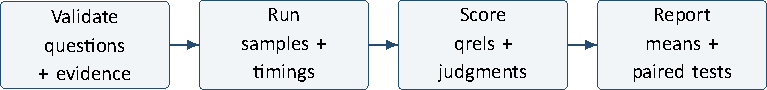
\includegraphics{figures/rendered/figure-05.pdf}
\caption{Independent benchmark workflow. Offline judging does not alter the stored inference answer.}\label{fig:benchmark}
\end{figure}

\section{Ethical Considerations}
The system presents information from supplied sources and is not a substitute for professional assessment of a specific dispute. It should not silently transform missing evidence into a confident legal conclusion. Source provenance and an explicit fallback help readers inspect the basis of an answer, but neither removes model error nor resolves the effective legal status of a source.

The evaluation set contains public legal-text questions rather than personal case files. Future deployment with user cases would need explicit handling of private information, retention, and access control. For the present report, the main ethical obligations are accurate attribution, transparent uncertainty, and faithful reporting of failures and judge limitations. No unsupported current-validity conclusion is inferred from an amendment edge or a completed pipeline status.
% END chapters/methodology

% BEGIN chapters/design
\chapter{System Design and Implementation}\label{ch:design}
\section{AI Model Integration}
The orchestration layer coordinates small, explicit components rather than placing all behaviour in one prompt. Query analysis produces structured intent, entities, and a retrieval rewrite. Deterministic code derives filters from the original request. The retrievers return ranked chunks through shared contracts. Context construction retains source evidence, while generation and verification use those retained sources as their common reference.

Table~\ref{tab:modules} maps the main responsibilities to the implementation. This division permits a component to be debugged with its input and output without invoking every model again. It also prevents the benchmark from acquiring a separate, subtly different implementation of answering logic.

\begin{table}[H]\centering\small
\caption{Implementation responsibilities and principal repository locations.}\label{tab:modules}
\begin{tabularx}{\textwidth}{P{3.2cm}Y}\toprule
\textbf{Responsibility} & \textbf{Code location, relative to repository root}\\\midrule
Runtime and index readiness & \path{src/runtime.py}\\
Source and corpus preparation & \path{src/data_pipeline/}\\
Query understanding and document references & \path{src/query_understanding/}\\
Lexical/dense retrieval and fusion & \path{src/retrieval/}\\
Document graph building and traversal & \path{src/knowledge_graph/}\\
Context packing and citation checks & \path{src/generation/}\\
Sufficiency decisions & \path{src/evaluation/retrieval_evaluator.py}\\
Pipeline state and feedback & \path{src/orchestration/rag_pipeline.py}\\
Independent benchmark & \path{src/benchmark/}, \path{scripts/benchmark.py}\\\bottomrule
\end{tabularx}
\end{table}

Model calls use role-specific prompts, structured response validation, timeouts, and bounded retry settings. In the recorded run, query analysis and citation verification use the 2B model, while context sufficiency and answer generation use the 4B model. The same family also supplies the offline judge at a different stage. Local serving simplifies access to the models, but shared-family judgments may have correlated errors and are not an independent correctness guarantee.

\section{Data Flow and Processing}
\subsection{Offline Preparation}
Preparation first resolves the source revision and selected topics, normalizes records, and constructs hierarchical chunks. Leaf embeddings are cached using chunk identity and text content. Prepared-corpus identity distinguishes the selected source and preparation configuration. A healthy existing prepared corpus can be reused; the runtime then checks index readiness rather than always recomputing embeddings and rewriting all database rows.

Leaf vectors are stored in PostgreSQL using pgvector HNSW cosine search with $m=16$, construction effort 128 and search effort 100. The observed configuration uses a connection pool of three. Neo4j stores source-backed document relationships and chunk hierarchy. Readiness checks and explicit reindex options are separate from source-refresh checks, so a query-prompt change does not by itself require corpus re-embedding.

\subsection{Online Question Answering}
Figure~\ref{fig:architecture} gives the actual stage order. Context sufficiency is evaluated \emph{before} generation. The feedback loop returns to retrieval only when the online decision calls for refinement and the round limit permits it. Graph traversal depth and the number of retrieval rounds are different controls.

\begin{figure}[H]\centering
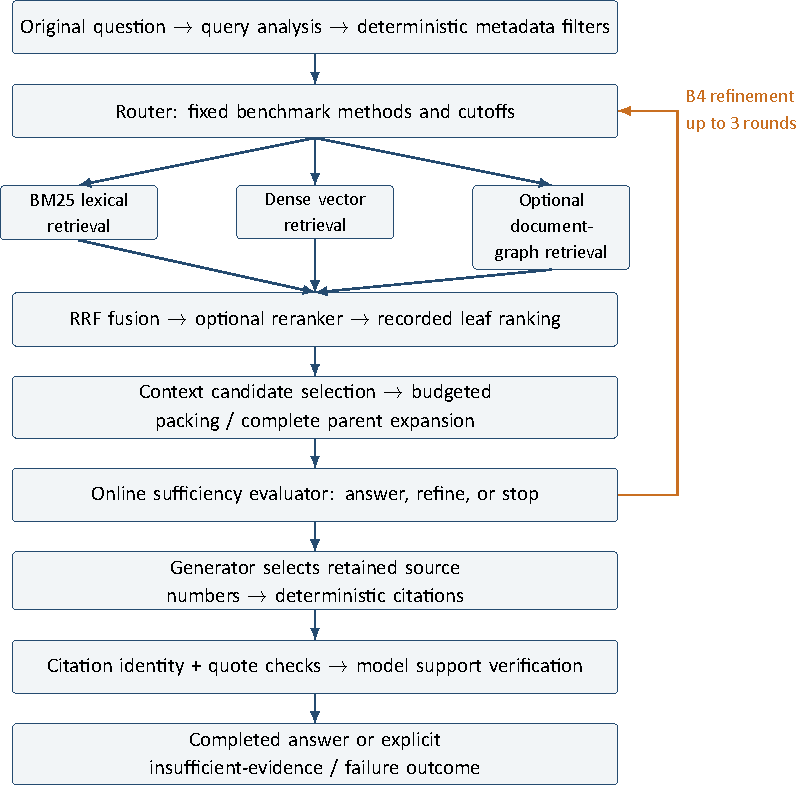
\includegraphics{figures/rendered/figure-06.pdf}
\caption{Implemented online architecture. Database preparation and offline benchmark judging are outside this inference flow.}\label{fig:architecture}
\end{figure}

The original question remains the controlling request throughout evaluation. The rewritten retrieval query is not substituted for it in the sufficiency judgment. This matters when a rewrite omits a requested document or narrows a conjunction into a single clause. Hard filters use deterministic reference resolution; the pipeline does not trust an LLM to silently redefine legal scope.

The context builder first prioritizes candidates relevant to explicit provision names and balances requested documents. It then packs leaves under the configured budget and considers complete parent expansion. Expansion must not evict other retained evidence, and it does not truncate a provision halfway through to fit a model window. These rules aim to preserve conditions and exceptions while preventing one long document from consuming all available context. They are shared by B0--B4.

The online evaluator decides whether the packed context is enough for the original question. If evidence is sufficient, the generator writes the response and selects numbered retained sources. If it is insufficient, B4 may refine retrieval; the other methods stop after their single round. The maximum of three rounds is a bound, not a requirement to run all three for every question.

\subsection{Document-Reference Graph}
The graph builder derives relationships from source metadata and explicit source references. Typed links include \code{AMENDS}, \code{REPLACES}, \code{REPEALS}, and \code{RELATED_TO}. Modification links point from the later modifying document to the earlier target. Unresolved references are retained for inspection rather than invented as fully resolved legal facts.

\begin{figure}[H]\centering
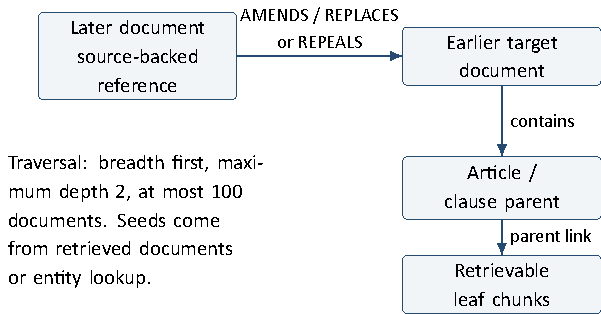
\includegraphics{figures/rendered/figure-07.pdf}
\caption{Graph schema and traversal bounds. Nodes illustrate types, not asserted links between named legal instruments.}\label{fig:graph}
\end{figure}

The retriever performs bounded breadth-first expansion. It ranks candidate chunks using lexical overlap, depth and stable identity tie-breaking. Graph candidates then pass through the common metadata and fusion rules. Explicit relation evidence must survive the retention checks before a relationship is included in packed context. Consequently, enabling graph traversal does not imply that a relation block reaches the answer generator. Chapter~\ref{ch:results} audits that distinction in the pilot.

\subsection{Generation, Verification and Failure Visibility}
Citation identities, provision locations, source URLs and verbatim quotations are derived from retained source objects after the generator chooses source numbers. This reduces opportunities for invented document numbers or quotations. The verifier checks identity and quote consistency deterministically, then asks a model to assess support using only actually cited retained sources. It does not silently repair an unsupported answer by dropping a citation.

The system records completed, insufficient-evidence, failed and timed-out outcomes separately. A verifier rejection is a failure outcome, not an answer-quality score. Structured failure stage, exception type and diagnostic information support debugging. Likewise, an inactive refinement hint may be normalized without changing the evaluator's decision; an inconsistent ``insufficient but continue'' decision is rejected rather than accepted as success.

The current citation contract operates at the answer and selected-source level. It does not establish a formal sentence-to-provision proof, and a completed status does not mean that every claim was correctly judged. The report therefore evaluates completion independently from faithfulness and reference-based factual scores.

\section{Deployment Strategy}
The reproducible local deployment consists of a Python environment, Ollama, PostgreSQL with pgvector, and Neo4j. The repository provides database startup and diagnostic commands. CLI preparation creates or reuses indexes; CLI answering and chat invoke the same orchestration components as the benchmark. Configuration files under \path{configs/demo/} define the runtime, while \path{configs/benchmark/} defines the experimental matrix and offline judge.

The recorded environment is Python 3.12.13 on Windows 11 build 10.0.26300. The manifest records an AMD64 Family 25 Model 68 Stepping 1 CPU descriptor, ONNX Runtime 1.31.1, NumPy 2.5.1, Pydantic 2.13.4, Neo4j driver 6.4.1 and psycopg 3.3.4. Exact CPU product name, RAM, GPU, LLM quantization and system load are not documented. The reranker export is known to be int8, which should not be generalized to the Ollama models.

An API host/port configuration is not evidence of a delivered web service. A browser UI, authentication layer, monitored production endpoint and automatic legal update workflow are not implemented capabilities demonstrated by this study. The deployment claim is limited to the local CLI prototype and its benchmark.

\section{Scalability and Maintenance}
Embedding caches, prepared-corpus identities, index reuse and atomic artifacts reduce repeated work. Interrupted benchmarks can resume compatible missing samples. Rescoring reuses stored answers under a recorded judge identity. These features improve maintainability; concurrent-user throughput remains unmeasured.

Future scaling studies should measure database search, model loading and decoding under controlled hardware and concurrency. Nested model and stage spans must not be double-counted. Source refresh and reindex procedures must preserve label-to-revision mappings so that changed data are not mistaken for a method improvement.
% END chapters/design

% BEGIN chapters/results
\chapter{Results and Discussion}\label{ch:results}
\section{Results and Analysis}
\subsection{Run Integrity and Coverage}
The analyzed run is \code{three-topics-dev-v1-fixed-01}. It contains all 225 expected samples and 225 score artifacts. The recorded report audit checks sample--score fingerprints, question and qrels alignment, recomputed retrieval metrics, aggregate breakdowns, paired statistics and Holm corrections, finite values, and quality/latency CSV exports. The numeric inputs in this report are exported from those frozen artifacts; they do not come from the earlier smoke test.

Every configuration completes 43 of 45 questions and returns insufficient evidence for GD014 and KHCN013. No inference execution is recorded as failed or timed out. Across configurations, this is 215 completed responses and ten insufficient-evidence outcomes. The 95.56\% completion rate describes workflow coverage, not answer accuracy.

\begin{figure}[H]\centering
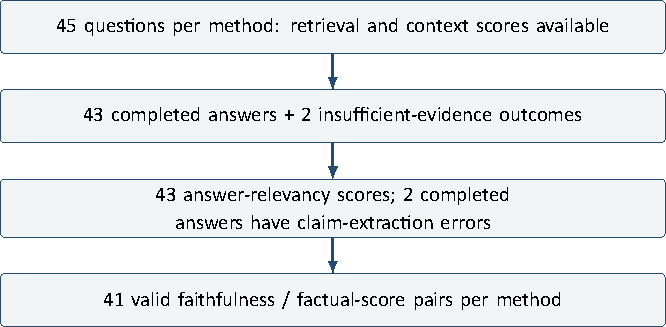
\includegraphics{figures/rendered/figure-08.pdf}
\caption{Metric availability per configuration. Different denominators prevent a single uniform ``accuracy'' interpretation.}\label{fig:availability}
\end{figure}

The two extraction-error questions are GT009 and GD015 in every configuration, giving ten judge-error samples overall. The judge output is truncated at its configured 2,048-token limit during answer-claim extraction. These are scoring errors on completed inference artifacts. They are not reclassified as inference failures, and missing claim-based scores are excluded rather than replaced with zero. Context metrics remain available for all 45 questions and answer relevancy for 43.

\subsection{Retriever Performance}
Table~\ref{tab:retrieval} reports macro means over all 45 questions for each method. Recall@5 is already high for the hybrid baseline, while B1, B3 and B4 obtain slightly higher observed recall. The small nDCG differences indicate changes near the top of an already strong ranking on this development set.

\begin{table}[H]\centering\small
\caption{Retrieval quality on 45 development questions. All values use binary leaf qrels.}\label{tab:retrieval}
\begin{tabular}{lrrrrrr}\toprule
\textbf{Method} & \textbf{R@5} & \textbf{P@5} & \textbf{MRR@5} & \textbf{MAP@5} & \textbf{nDCG@5} & \textbf{R@20}\\\midrule
% BEGIN data/retrieval-table.tex
B0 & 0.9667 & 0.2133 & 0.9630 & 0.9359 & 0.9508 & 0.9889 \\
B1 & 0.9778 & 0.2178 & 0.9656 & 0.9461 & 0.9587 & 0.9889 \\
B2 & 0.9667 & 0.2133 & 0.9741 & 0.9415 & 0.9559 & 0.9889 \\
B3 & 0.9778 & 0.2178 & 0.9674 & 0.9470 & 0.9596 & 0.9889 \\
B4 & 0.9778 & 0.2178 & 0.9711 & 0.9489 & 0.9614 & 1.0000 \\
% END data/retrieval-table.tex

\bottomrule\end{tabular}
\note{Precision@5 has a dataset-label ceiling of 0.2267; the reference labels are not exhaustive judgments of every useful passage.}
\end{table}

\begin{figure}[H]\centering
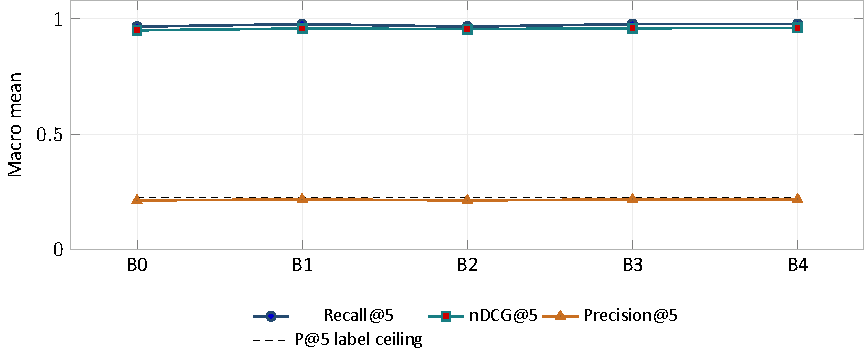
\includegraphics{figures/rendered/figure-09.pdf}
\caption{High labeled-evidence recall coexists with a low numeric precision ceiling. Lines connect configurations for readability, not a continuous parameter.}\label{fig:retrieval}
\end{figure}

B0 obtains Recall@5 of 0.9667 and P@5 of 0.2133. The reranked variants reach 0.9778 and 0.2178. Against the qrels ceiling, those precision values represent most of the possible top-five relevant-label count. It would be incorrect to diagnose a 78\% answering error rate from $1-P@5$, because the denominator is five retrieved ranks and most questions label only one leaf.

B4 reaches Recall@20 of 1.0000, yet still does not complete the two rejected questions. Retrieval recall and answer sufficiency therefore diverge in an observable way: finding the labeled leaf IDs somewhere in a ranked list is not equivalent to retaining all required context or obtaining a correct gate decision.

\subsection{Packed Context and Answer Quality}
\begin{table}[H]\centering\small
\caption{Context and answer metrics from the current offline judge. These are provisional measurements.}\label{tab:quality}
\begin{tabular}{lrrrrr}\toprule
\textbf{Method} & \textbf{Context P} & \textbf{Context R} & \textbf{Faithfulness} & \textbf{Factual F1} & \textbf{Answer rel.}\\\midrule
% BEGIN data/quality-table.tex
B0 & 0.9909 & 0.8138 & 0.6153 & 0.4905 & 0.6880 \\
B1 & 0.9963 & 0.7697 & 0.6234 & 0.4480 & 0.6915 \\
B2 & 0.9854 & 0.8305 & 0.6267 & 0.5062 & 0.6888 \\
B3 & 0.9963 & 0.7753 & 0.6295 & 0.4508 & 0.6922 \\
B4 & 0.9963 & 0.7708 & 0.6295 & 0.4508 & 0.6922 \\
% END data/quality-table.tex

\bottomrule\end{tabular}
\note{Valid questions per method: Context P/R $n=45$; faithfulness and factual F1 $n=41$; answer relevancy $n=43$. Higher is better within each metric, but their units and denominators differ.}
\end{table}

Context Precision ranges from 0.9854 to 0.9963, while Context Recall ranges from 0.7697 to 0.8305. This is consistent with a context collection that the judge finds useful early in its order but not necessarily complete against all reference claims. High rank-aware context precision should not be interpreted as evidence that every clause needed by the question is present.

B2 has the largest observed Context Recall and Factual F1 means, whereas B3 and B4 have the largest faithfulness and answer-relevancy means. B1 increases retrieval Recall@5 relative to B0 but has a lower judged factual F1. These descriptive differences show why ranking and answer scores must both be inspected. They do not prove which component caused a particular judgment, especially given the judge errors discussed below.

\begin{figure}[H]\centering
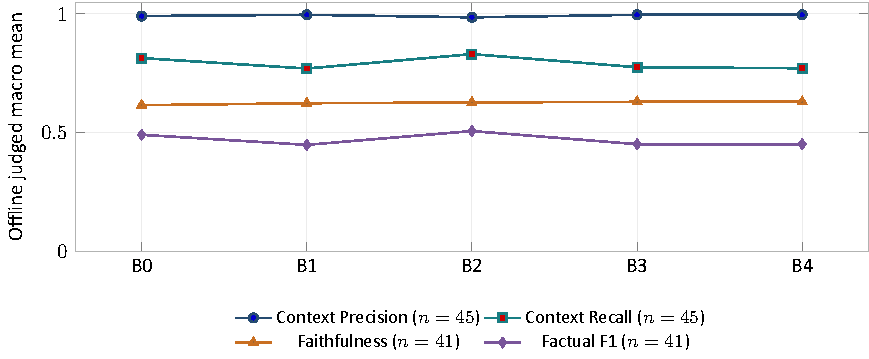
\includegraphics{figures/rendered/figure-10.pdf}
\caption{Stage-specific quality profiles. Judge calibration is required before treating these answer scores as reliable legal-correctness estimates.}\label{fig:quality}
\end{figure}

The additional claim-precision, claim-recall and strict-yield results appear in Table~\ref{tab:factual}. Near-zero strict yield follows from requiring two imperfect judge measures to equal one simultaneously. It should not be described as evidence that nearly all answers are wrong.

\begin{table}[H]\centering\small
\caption{Reference-based claim scores and strict correct-answer yield.}\label{tab:factual}
\begin{tabular}{lrrrr}\toprule
\textbf{Method} & \textbf{Factual P} & \textbf{Factual R} & \textbf{Factual F1} & \textbf{Strict yield}\\\midrule
% BEGIN data/factual-table.tex
B0 & 0.5753 & 0.6813 & 0.4905 & 0.0233 \\
B1 & 0.5350 & 0.6716 & 0.4480 & 0.0000 \\
B2 & 0.5928 & 0.6935 & 0.5062 & 0.0465 \\
B3 & 0.5411 & 0.6675 & 0.4508 & 0.0000 \\
B4 & 0.5411 & 0.6675 & 0.4508 & 0.0000 \\
% END data/factual-table.tex

\bottomrule\end{tabular}
\note{Claim metrics use 41 valid completed answers. Yield uses 43 valid outcomes, including the two insufficient-evidence zeros and excluding two judge-error answers.}
\end{table}

\subsection{Paired Uncertainty}
No reported test reaches a Holm-adjusted $p<0.05$. Figure~\ref{fig:ci} displays the paired nDCG@5 deltas relative to B0. For B3--B0, the mean difference is 0.0088 with a pointwise 95\% interval of $[-0.0124,0.0347]$ and adjusted $p=1.000$. This does not substantiate a retrieval advantage over the baseline.

\begin{figure}[H]\centering
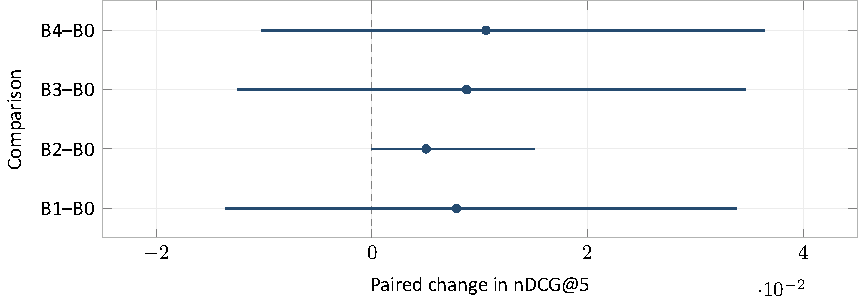
\includegraphics{figures/rendered/figure-11.pdf}
\caption{Point estimates and pointwise 95\% paired bootstrap intervals ($n=45$, 2,000 resamples). All four Holm-adjusted tests have $p=1.000$; intervals are not simultaneous family-adjusted intervals.}\label{fig:ci}
\end{figure}

B2's factual F1 delta relative to B0 is 0.0157 on 41 paired valid questions, with pointwise interval $[0.0000,0.0423]$ and adjusted $p=1.000$. A non-negative pointwise interval is not sufficient to declare a winner when the reported multiple-comparison procedure does not reject the null. Conversely, failing to find significance is not proof of equivalence. The experiment is small, development-tuned and judged by a model that still needs calibration.

\subsection{Inference Latency}
\begin{table}[H]\centering\small
\caption{Full-pipeline wall-clock latency in seconds. Preparation and offline scoring are excluded.}\label{tab:latency}
\begin{tabular}{lrrrr}\toprule
\textbf{Method} & \textbf{All mean} & \textbf{Completed mean} & \textbf{Completed p50} & \textbf{Completed p95}\\\midrule
% BEGIN data/latency-table.tex
B0 & 21.76 & 22.00 & 21.40 & 27.65 \\
B1 & 23.04 & 23.14 & 21.86 & 32.42 \\
B2 & 22.13 & 22.37 & 21.76 & 28.30 \\
B3 & 23.27 & 23.48 & 22.23 & 31.35 \\
B4 & 24.28 & 23.44 & 22.08 & 31.88 \\
% END data/latency-table.tex

\bottomrule\end{tabular}
\note{All mean uses $n=45$; completed-only statistics use $n=43$ per method. Percentiles use the benchmark's linear interpolation convention. These are measurements on one incompletely described local machine.}
\end{table}

B0 has the lowest observed all-outcome mean at 21.76 seconds. B1, B2 and B3 average 23.04, 22.13 and 23.27 seconds. B4 averages 24.28 seconds, approximately 11.6\% above B0 in this run. These values describe the recorded local execution; one repeat and incomplete hardware notes do not support a portable latency guarantee.

\begin{figure}[H]\centering
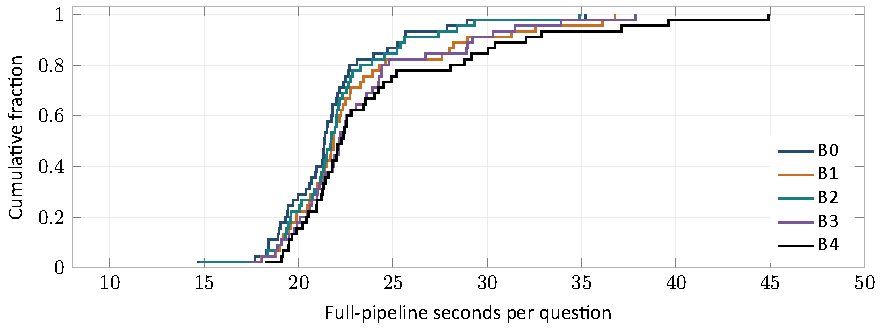
\includegraphics{figures/rendered/figure-12.pdf}
\caption{Empirical latency distributions over all 45 outcomes per method, including insufficient-evidence cases. Curves show observations rather than fitted distributions.}\label{fig:latency}
\end{figure}

The completed-only means for B3 and B4 are very similar. Their difference in all-outcome mean is driven by extra work on the rejected questions: B4's two insufficient-evidence outcomes average 42.25 seconds, compared with 18.78 seconds for B3. It is therefore important to include those outcomes when describing the operational cost of feedback. Reporting completed-only speed would hide the additional unsuccessful retrieval rounds.

\subsection{Feedback and Graph Observations}
In B4, 43 questions stop after one retrieval round and two run all three rounds. The total is 49 rounds, compared with 45 for each single-round method. All 45 final answer objects are identical between B3 and B4. Feedback changes some deeper ranking results, including Recall@20, but recovers no additional completed answer in this pilot.

The graph branch is enabled in B2, B3 and B4. Inspection of stored retrieval rounds finds zero retained relation lists in the final ranked retrieval results for all methods, and zero explicit document-relation blocks in final context text. This does not mean the prepared graph has no relationships or that the enabled branch could not affect candidate ranks. It does mean that the pilot provides no evidence of answering with an explicit retained graph-relation block. Graph-assisted candidate retrieval and demonstrated graph-grounded multi-hop reasoning are different claims.

Mean packed-context sizes are approximately 1,489 tokens for B0, 1,498 for B1, 1,476 for B2, 1,498 for B3 and 1,504 for B4. These averages are below the configured context ceiling, but do not establish that every needed provision was available or selected. A larger budget alone cannot fix a wrong candidate or an overly demanding gate.

\section{Discussion}
\subsection{Why Completion Is Not Accuracy}
The absence of inference failures is a useful engineering result. The revised contracts can finish the complete B0--B4 workflow and preserve inspectable artifacts. Nevertheless, the remaining insufficient-evidence cases and quality-judge issues prevent a claim of 95.56\% legal accuracy. Completed responses still require evidence-level review, and a fallback can be appropriate when the requested facts are not retained.

The two rejected questions illustrate different bottlenecks. For GD014, the packed material misses the general scope provision of the Education Law and emphasizes narrower adult-education and policy provisions. Rejecting that context can be justified by the missing scope. For KHCN013, the retained material includes the three appendices and the clause concerning proposals to update the list, but the online evaluator demands additional procedural deadlines and documents beyond the requested detail. This suggests a possible false-negative sufficiency judgment. It is not evidence that the generator should always be allowed to answer after a failed gate.

\subsection{Why the Offline Scores Need Calibration}
The stored judgments permit direct counterexamples to a literal reading of faithfulness. In B0/GD001, the answer and the retained scope provision both enumerate the education system, educational institutions, teachers, learners, state management, and associated rights and responsibilities. The judge nevertheless reports faithfulness of 0.3333 while factual F1 is 1.0000. Its reasons demand detailed provisions or confirmation of current validity that the scope statement does not assert.

In B0/GT002, the answer states the applicable organizations and individuals for inland-waterway activity, with a treaty condition. The factual judge rejects part of the answer using a reason about other transport modes that the response does not claim. These cases demonstrate semantic judging errors. They do not show that every low score is erroneous, nor establish an adjusted true score.

Claim extraction is also a source of error: removing the relation ``the law regulates'' can turn a supported statement about scope into a fragmented statement that the entailment judge interprets differently. GT009's extraction truncation occurs even though its final response is only about 318 characters. Increasing the token limit might reduce a particular failure, but would not by itself demonstrate stable or valid claim decomposition. The required next step is calibrated extraction and entailment against human-reviewed examples, followed by rescoring the same frozen answers.

\begin{table}[H]\centering\small
\caption{Observed issues separated by pipeline or measurement stage.}\label{tab:issues}
\begin{tabularx}{\textwidth}{P{2.3cm}P{3cm}Y}\toprule
\textbf{Case} & \textbf{Stage} & \textbf{Evidence and interpretation}\\\midrule
GD014 & Retrieval / context & General scope not retained; missing evidence can explain fallback.\\
KHCN013 & Online sufficiency & Evaluator requests details beyond the asked scope; possible false negative.\\
GT009, GD015 & Offline extraction & Truncation in all methods; claim-based scores unavailable.\\
B0/GD001 & Offline entailment & Same scope information receives low faithfulness but perfect factual F1.\\
B0/GT002 & Offline factual judgment & Rejection reason introduces transport modes absent from the response.\\\bottomrule
\end{tabularx}
\end{table}

\subsection{Threats to Validity}
\textbf{Construct validity.} Binary leaf labels, rank-aware context precision and claim-based quality scores represent different constructs. None is a complete measure of legal correctness. Incomplete alternative-evidence labeling constrains the interpretation of precision, and model judgments introduce prompt- and model-dependent error.

\textbf{Internal validity.} The ablation shares corpus, models, filters and budgets, which supports comparison. However, a component changes the downstream evidence seen by common stages, so aggregate changes cannot be attributed to one isolated mechanism without trace analysis. Near-ceiling retrieval and a single repeat reduce sensitivity to small gains. Development fixes and question clarifications also prevent an unbiased final-test interpretation.

\textbf{External validity.} Only three topics and 45 answerable questions are included. Explicit document and title cues make some questions easier to constrain than broad real-user requests. Few questions are comparisons or multi-document tasks, and the run includes no held-out unanswerable or adversarial temporal cases. Generalization to open-ended legal consultation or graph-dependent reasoning remains untested.

\textbf{Measurement reliability.} Some judge outputs are invalid and others semantically inconsistent. Local hardware and LLM quantization records are incomplete. A technically correct aggregation can faithfully summarize unreliable judgments; arithmetic consistency and semantic validity must therefore be audited separately.

\clearpage
\section{Recommendations}
The first priority is to stabilize claim extraction and calibrate the offline judge on a stratified, independently reviewed subset. Reviewers should preserve conditions, exceptions and the original question's scope. Agreement, error categories, and examples should be documented before introducing a new judge identity and rescoring the existing inference artifacts.

The second priority is a reviewed dataset with a development/test boundary established before further tuning. It should include alternative supporting provisions where relevant, more multi-document questions requiring real graph links, and unanswerable cases. Topic balance alone is insufficient; task difficulty, evidence multiplicity, document age and ambiguity should also be characterized. Negative controls should test whether related but insufficient provisions are correctly rejected.

The third priority is a controlled repeated experiment with complete CPU/GPU/RAM, model digest, quantization, database and load records. Paired comparisons should be planned in advance with a small set of primary metrics. B0 remains the simplest reference configuration for continued development because it has the lowest observed mean latency and strong retrieval here. This is an engineering choice for the next experiment, not a statistically established quality winner.

For graph research, instrument the number of graph-only relevant hits, retained relation evidence, and genuinely graph-dependent questions. For feedback, distinguish recovery of missing evidence from repeated rejection of already adequate context. These measurements would explain \emph{when} an addition helps, which is more informative than enabling it by default because it increases architectural complexity.
% END chapters/results

% BEGIN chapters/conclusion
\chapter{Conclusion}\label{ch:conclusion}
\section{Summary of Findings}
The project delivers a local Vietnamese legal RAG prototype and a separate benchmark workflow. It combines hybrid retrieval, optional graph expansion and reranking, hierarchical context, pre-generation sufficiency evaluation, source-derived citations and post-generation verification. Models remain pretrained and the graph uses source-backed document references.

The development study covers 45 questions, three topics and five configurations, with 225 complete inference records. Each method completes 43 questions and returns insufficient evidence for two; no inference failure or timeout is recorded. Retrieval Recall@5 ranges from 0.9667 to 0.9778 and nDCG@5 from 0.9508 to 0.9614. Precision@5 ranges from 0.2133 to 0.2178 against a label-defined ceiling of 0.2267. These results support strong retrieval of the specified labels on this development set, not universal legal-question accuracy.

The optional components do not establish a statistically significant quality advantage under the reported Holm-adjusted comparisons. B0 has the lowest observed all-outcome mean inference latency at 21.76 seconds; B4 has the highest at 24.28 seconds. B4's additional rounds recover no extra completed answers, and its final answers match B3 for all 45 questions. No explicit graph-relation block survives into packed context in the recorded pilot, so a graph-grounded multi-hop benefit is not demonstrated.

\section{Contributions and Reflections on the Project}
The engineering contribution is a pipeline with visible evidence boundaries and failure states. Controlled method switches, source-resolved qrels, separate scoring artifacts, configuration identities, telemetry and paired statistics make its results inspectable, including when additions do not outperform the baseline.

The methodological lesson is that an operational benchmark is not automatically a valid correctness measure. This run is complete and arithmetically auditable, yet its judge has truncation errors and incorrect entailment decisions. Low faithfulness means cannot be converted directly into a hallucination rate.

\section{Limitations and Future Work}
The current set has informed development, contains only answerable questions, and awaits independent legal review. Its evidence labels are narrow, its task mix is dominated by lookup and multi-clause questions, and it has only one repeat per configuration. Hardware and LLM quantization records are incomplete. Neither a current-validity service nor a production web application is established by this implementation.

Future work should calibrate the judge against reviewed labels and rescore the frozen answers. A larger held-out test should include graph-dependent, multi-document, ambiguous and unanswerable requests. Repeated runs with complete environment records are needed before stronger comparative or deployment claims.
% END chapters/conclusion

\chapter{References}
\begingroup
\renewcommand{\bibsection}{}
\small\setlength{\bibsep}{5pt}
\begin{thebibliography}{10}
\providecommand{\natexlab}[1]{#1}
\providecommand{\url}[1]{\texttt{#1}}
\expandafter\ifx\csname urlstyle\endcsname\relax
  \providecommand{\doi}[1]{doi: #1}\else
  \providecommand{\doi}{doi: \begingroup \urlstyle{rm}\Url}\fi

\bibitem[Chen et~al.(2024)Chen, Xiao, Zhang, Luo, Lian, and Liu]{chen2024m3}
Jianlv Chen, Shitao Xiao, Peitian Zhang, Kun Luo, Defu Lian, and Zheng Liu.
\newblock {M3}-embedding: Multi-linguality, multi-functionality,
  multi-granularity text embeddings through self-knowledge distillation.
\newblock \emph{arXiv preprint arXiv:2402.03216}, 2024.
\newblock \doi{10.48550/arXiv.2402.03216}.
\newblock URL \url{https://arxiv.org/abs/2402.03216}.

\bibitem[Cormack et~al.(2009)Cormack, Clarke, and B{\"u}ttcher]{cormack2009rrf}
Gordon~V. Cormack, Charles L.~A. Clarke, and Stefan B{\"u}ttcher.
\newblock Reciprocal rank fusion outperforms condorcet and individual rank
  learning methods.
\newblock In \emph{Proceedings of the 32nd International ACM SIGIR Conference},
  pages 758--759, 2009.
\newblock \doi{10.1145/1571941.1572114}.
\newblock URL
  \url{https://cormack.uwaterloo.ca/cormack/cormacksigir09-rrf.pdf}.

\bibitem[Edge et~al.(2024)Edge, Trinh, Cheng, Bradley, Chao, Mody, Truitt,
  Metropolitansky, Ness, and Larson]{edge2024graph}
Darren Edge, Ha~Trinh, Newman Cheng, Joshua Bradley, Alex Chao, Apurva Mody,
  Steven Truitt, Dasha Metropolitansky, Robert~Osazuwa Ness, and Jonathan
  Larson.
\newblock From local to global: A graph {RAG} approach to query-focused
  summarization.
\newblock \emph{arXiv preprint arXiv:2404.16130}, 2024.
\newblock \doi{10.48550/arXiv.2404.16130}.
\newblock URL \url{https://arxiv.org/abs/2404.16130}.

\bibitem[Es et~al.(2024)Es, James, Espinosa~Anke, and Schockaert]{es2024ragas}
Shahul Es, Jithin James, Luis Espinosa~Anke, and Steven Schockaert.
\newblock {RAGAs}: Automated evaluation of retrieval augmented generation.
\newblock In \emph{Proceedings of the 18th Conference of the European Chapter
  of the Association for Computational Linguistics: System Demonstrations},
  pages 150--158. Association for Computational Linguistics, 2024.
\newblock \doi{10.18653/v1/2024.eacl-demo.16}.
\newblock URL \url{https://aclanthology.org/2024.eacl-demo.16/}.

\bibitem[J{\"a}rvelin and Kek{\"a}l{\"a}inen(2002)]{jarvelin2002gain}
Kalervo J{\"a}rvelin and Jaana Kek{\"a}l{\"a}inen.
\newblock Cumulated gain-based evaluation of {IR} techniques.
\newblock \emph{ACM Transactions on Information Systems}, 20\penalty0
  (4):\penalty0 422--446, 2002.
\newblock \doi{10.1145/582415.582418}.
\newblock URL \url{https://doi.org/10.1145/582415.582418}.

\bibitem[Lewis et~al.(2020)Lewis, Perez, Piktus, Petroni, Karpukhin, Goyal,
  K{\"u}ttler, Lewis, Yih, Rockt{\"a}schel, Riedel, and Kiela]{lewis2020rag}
Patrick Lewis, Ethan Perez, Aleksandra Piktus, Fabio Petroni, Vladimir
  Karpukhin, Naman Goyal, Heinrich K{\"u}ttler, Mike Lewis, Wen-tau Yih, Tim
  Rockt{\"a}schel, Sebastian Riedel, and Douwe Kiela.
\newblock Retrieval-augmented generation for knowledge-intensive {NLP} tasks.
\newblock In \emph{Advances in Neural Information Processing Systems},
  volume~33, pages 9459--9474, 2020.
\newblock URL \url{https://arxiv.org/abs/2005.11401}.

\bibitem[Robertson and Zaragoza(2009)]{robertson2009bm25}
Stephen Robertson and Hugo Zaragoza.
\newblock The probabilistic relevance framework: {BM25} and beyond.
\newblock \emph{Foundations and Trends in Information Retrieval}, 3\penalty0
  (4):\penalty0 333--389, 2009.
\newblock \doi{10.1561/1500000019}.
\newblock URL
  \url{https://www.nowpublishers.com/article/DownloadEBook/INR-019}.

\bibitem[Saad-Falcon et~al.(2024)Saad-Falcon, Khattab, Potts, and
  Zaharia]{saadfalcon2024ares}
Jon Saad-Falcon, Omar Khattab, Christopher Potts, and Matei Zaharia.
\newblock {ARES}: An automated evaluation framework for retrieval-augmented
  generation systems.
\newblock In \emph{Proceedings of the 2024 Conference of the North American
  Chapter of the Association for Computational Linguistics: Human Language
  Technologies (Volume 1: Long Papers)}, pages 338--354. Association for
  Computational Linguistics, 2024.
\newblock \doi{10.18653/v1/2024.naacl-long.20}.
\newblock URL \url{https://aclanthology.org/2024.naacl-long.20/}.

\bibitem[{Sentence Transformers}(n.d.)]{mmarco}
{Sentence Transformers}.
\newblock Cross-encoder for multilingual {MS MARCO}: Model card, n.d.
\newblock URL
  \url{https://huggingface.co/cross-encoder/mmarco-mMiniLMv2-L12-H384-v1}.
\newblock Accessed 5 November 2026; experiment revision
  1427fd652930e4ba29e8149678df786c240d8825.

\bibitem[{tmquan}(n.d.)]{phapdien}
{tmquan}.
\newblock Phapdien ministry of justice legal-text dataset: Community mirror,
  n.d.
\newblock URL \url{https://huggingface.co/datasets/tmquan/phapdien-moj-gov-vn}.
\newblock Accessed 5 November 2026; resolved source revision
  a1b6860c821b7142ffe2385178af4e4bb6f86aff.

\end{thebibliography}

\endgroup
% BEGIN chapters/appendices
\chapter{Appendices}\label{ch:appendices}
\section{Reproduction Guide: Windows CMD and Conda}
The commands below are for Windows CMD from the repository root. They assume Conda is installed and the project dependencies, Ollama models and database services are available. The existing environment name \code{free_env} is the one used in the recorded workflow. On another machine, activate the environment in which the project is installed. Full installation and database instructions remain in \path{docs/BENCHMARK_QUICKSTART.md}.

\begin{commands}
conda activate free_env
cd /d D:\dsp-vietnamese-legal-rag
python -m pip install -e ".[dev]"
ollama pull bge-m3
ollama pull qwen3.5:2b
ollama pull qwen3.5:4b
powershell -ExecutionPolicy Bypass -File scripts\start_demo_databases.ps1
\end{commands}
The default demo configuration selects the three topics used in this report. Remove any overrides left from the national-security smoke example in the quick-start document; keep all prepare/run/score commands in the same terminal. The subject override below ensures that selection is not narrowed by a previous session. Pin the source revision before preparation.
\begin{commands}
set RAG__DATA_PIPELINE__SOURCE__TOPICS=
set RAG__DATA_PIPELINE__SOURCE__SUBJECTS=[]
set RAG__DATA_PIPELINE__SOURCE__REVISION=a1b6860c821b7142ffe2385178af4e4bb6f86aff
python -m scripts.demo doctor
python -m scripts.demo prepare
\end{commands}
Preparation is outside the inference measurement and may be expensive on first use. It reuses prepared embeddings and healthy indexes on subsequent runs. The database startup script writes local credentials under \path{.runtime/demo.env}; credentials and model caches should not be committed or copied into the report package.

Validate the normalized development dataset and use a new output directory for a new inference run. The supplied \path{reports/latex/recorded-pilot.yml} preserves the one-repeat experiment matrix that produced the reported numbers. Its hardware-note placeholder records missing information and must be filled accurately before a new performance study.
\begin{commands}
python -m scripts.benchmark validate --dataset data\evaluation\new\three_topics_pilot.development.v1.jsonl
set BENCH_OUT=.runtime\benchmarks\three-topics-dev-next-01
python -m scripts.benchmark run --dataset data\evaluation\new\three_topics_pilot.development.v1.jsonl --split development --config reports\latex\recorded-pilot.yml --output %BENCH_OUT%
python -m scripts.benchmark score --output %BENCH_OUT% --judge-config configs\benchmark\judging.yml
python -m scripts.benchmark report --output %BENCH_OUT%
\end{commands}
Run performs evidence resolution against the prepared corpus before inference. Reuse an output directory only for a compatible interrupted run; changed code, labels, models or configuration require a new directory. The ordinary \path{configs/benchmark/hybrid.yml} requests three repeats and is appropriate for a larger planned study, but it is not the one-repeat protocol summarized here.

To rebuild this report's tables from the frozen run without calling any model:
\begin{commands}
python reports\latex\export_data.py --run .runtime\benchmarks\three-topics-dev-v1-fixed-01
\end{commands}
The LaTeX source package includes the already exported data. A reader can compile the report without possessing the large local benchmark directory. Re-exporting from another run requires updating the narrative, denominators and case studies; it must not be treated as a blind document refresh.

\section{Artifact Inventory and Provenance}
\begin{table}[H]\centering\small
\caption{Artifacts supporting the reported experiment and reproducible document.}\label{tab:artifacts}
\begin{tabularx}{\textwidth}{P{4.2cm}Y}\toprule
\textbf{Artifact} & \textbf{Purpose}\\\midrule
\path{manifest.json} & Question contents, settings, experiment protocol, code and model identities.\\
\path{qrels.json} & Resolved relevant leaf IDs for exact source evidence.\\
\path{samples/<method>/*.json} & Final results, round rankings, packed context, status and telemetry.\\
\path{scores/<method>/*.json} & Metrics, extracted claims, judgments and scoring errors.\\
\path{reports/summary.json} & Denominators, breakdowns, paired intervals and adjusted tests.\\
\path{reports/summary.csv}, \path{reports/latency.csv} & Machine-readable quality and timing summaries.\\
\path{reports/report-audit.json} & Recalculation and artifact-consistency audit.\\
LaTeX \path{data/provenance.json} & Input SHA-256 hashes, metric denominators and compact trace findings.\\
LaTeX \path{data/metrics.csv}, \path{data/latency.csv} & Frozen numeric inputs for vector plots and tables.\\\bottomrule
\end{tabularx}
\end{table}
The benchmark manifest fingerprint is
\begin{quote}\footnotesize\path{0e1e282ab37d27309f76b6dbcff37dedb9cd7082641c9d7d1948142a87c717f2}.\end{quote}
Source revision and corpus identity are provided in Chapter~\ref{ch:methodology}. Dataset, run and scoring identities should be preserved together; a final answer alone cannot reveal whether a changed score came from inference, labels or the judge.

\section{Question Format and Review Rules}
A benchmark question must specify the requested scope and retain stable source evidence. Reference claims should be self-contained and preserve conditions, negation and exceptions. A list can remain one claim when all its items share a legal relation; fragmenting it into unrelated noun phrases may distort entailment. Evidence quotations must be continuous source text and must not be rewritten as explanations.

For a record such as GD001, the user asks what falls within the scope of document 43/2019/QH14. The reference statement concerns that law's scope, not a demand to reproduce every detailed provision about every listed subject. A reviewer should judge whether the answer preserves that relation and list, rather than adding requirements for current-validity analysis absent from the request. This example explains an annotation principle; it does not replace expert review of the full dataset.

The next evaluation version should document a legal reviewer, review date, snapshot revision, alternative valid sources, and resolution of disagreements. Questions used for tuning should stay in development. Final-test questions should remain unseen until the pipeline and judge protocol are fixed. Unanswerable labels should describe genuinely unsupported requests in the snapshot, not merely questions that the current retriever fails to solve.

\section{Interpretation Checklist}
Before presenting a comparison, verify that all methods used the same source corpus and relevant runtime settings; that every expected artifact is present; and that both sample statuses and metric denominators are visible. Then distinguish direct source-label retrieval measurements from model judgments, and inspect paired uncertainty rather than sorting rounded means.

For this study, the defensible statement is that a complete development benchmark is operational and the hybrid baseline retrieves most labeled evidence. The optional additions have not demonstrated a robust quality advantage. The evidence does not justify claims of near-zero hallucination, production readiness, comprehensive legal validity tracking, or graph-grounded multi-hop superiority. These boundaries are part of the result rather than omissions to hide in a future deployment.
% END chapters/appendices

\end{document}
